\documentclass{article}
\usepackage{pgfplots}

\begin{document}

\begin{figure}[h]
    \centering
    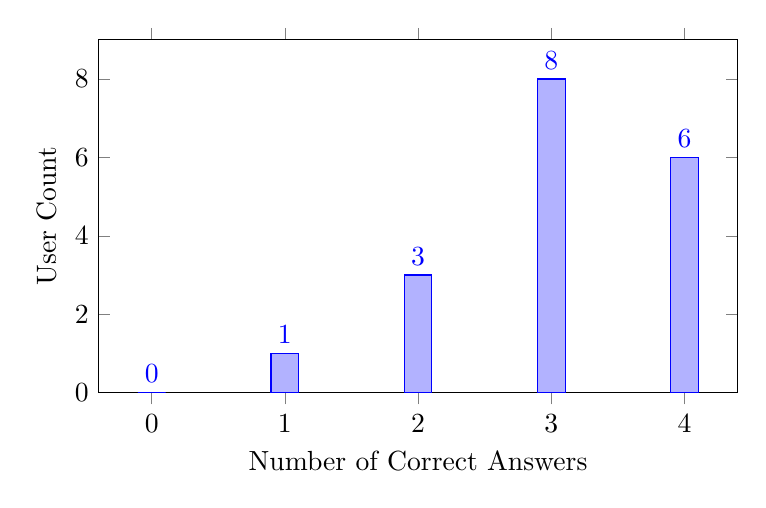
\begin{tikzpicture}
        \begin{axis}[
            ybar,
            ylabel={User Count},
            xlabel={Number of Correct Answers},
            symbolic x coords={0, 1, 2, 3, 4},
            xtick=data,
            nodes near coords,
            nodes near coords align={vertical},
            ymin=0,
            ymax=9,
            width=0.8\textwidth,
            height=0.5\textwidth,
            ]
            \addplot coordinates {(0,0) (1,1) (2,3) (3,8) (4,6)};
        \end{axis}
    \end{tikzpicture}
    \caption{Results of the user study. We report the number of correct answers, out of four questions, for all 18 participants. Amongst the 10 participants, none answered correctly less than 2 out of 4 questions, 2 participants answered correctly to exactly 2 questions, 4 participants correctly answered 3 questions, and 4 participants correctly answered to all 4 questions.}
    \label{fig:user_study_results}
\end{figure}

\end{document}